\chapter{Hardware}
Each unit is described by the following procedure:
\begin{itemize}
\item Overall design and block description - Quick design overview
\item Block breakdown - Detailed design overview
\item Block construction - Detailed implementation, simulation and calculation results.
\end{itemize}
This procedure is meant to ease readability and help give an overview of the entire system implementation.
\section{CDU}
The CDU responsibility is, as described in the previous documents, to control the custom powerline communication and to govern the information about the sensor nodes. The information is stored in memory and can be loaded out to a PC.
\subsection{Overall design}
The conceptual design of the CDU can be found in the architecture documentation in chapter Structural view, subsubsection CDU.\\
We take each block and create a block breakdown diagram.\\

\subsection{Block breakdown}
This section describes the interfaces and the design of each individual block.\\
Below, in figure \ref{fig:detailedCDU}, is shown a detailed overview of the CDU design. This will be the basis of the block breakdown section.
\begin{figure}[H]
	\centering
	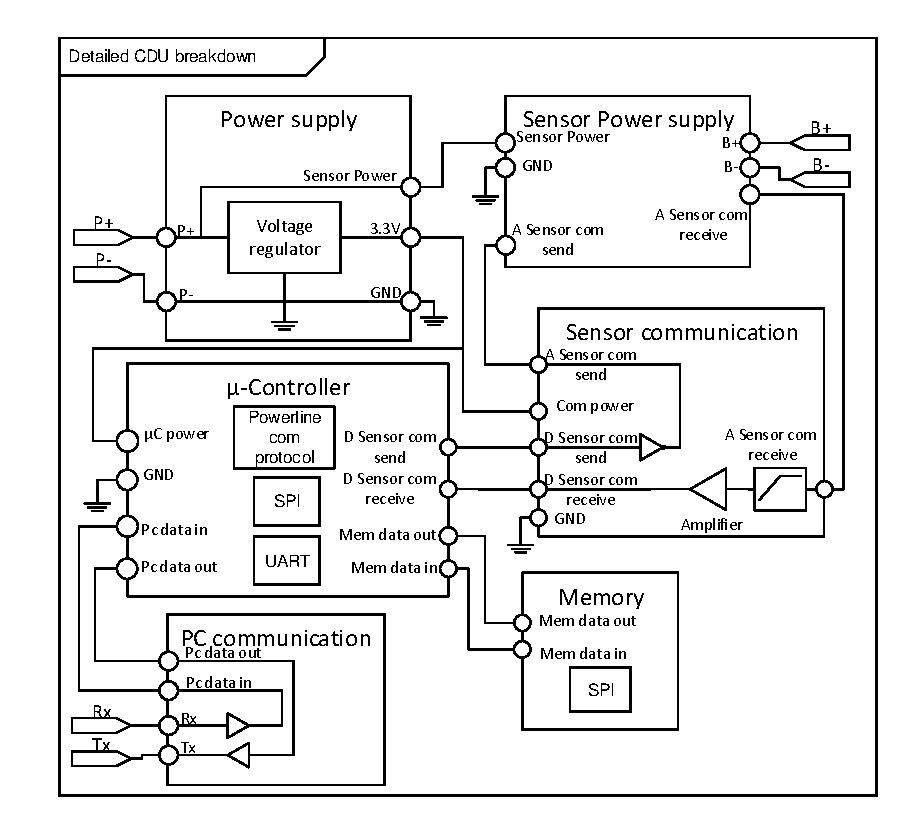
\includegraphics[width=1\textwidth]{billeder/detailedCDU}
	\caption{Detailed CDU breakdown}
	\label{fig:detailedCDU}
\end{figure}

The following subsections will cover all interfaces and design considerations.
\subsubsection{Power supply}
The Power supply is responsible for providing power to the internal circuitry and the powerline communication. 3.3V is provided for the internal circuitry. The voltage provided to the bus is determined by number of sensors and the sensor power supply circuit. The minimum voltage needed on P+ and P- pins is found by using the following formula: $( 5.5V - 0.7V ) + (5V * n + 0.7V) -> 5.5V + 5V * n$. The first parenthesis is the sensor power supply circuit and the second parenthesis is the bus voltage.\\
The interfaces to this block can be seen on figure ~\ref{fig:CDUPS}.\\
\begin{figure}[H]
	\centering
	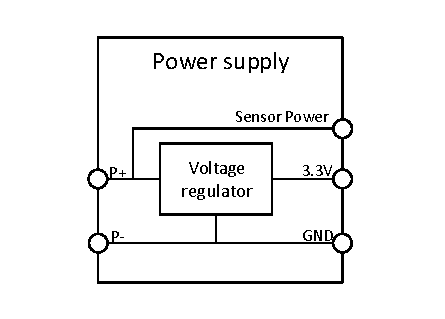
\includegraphics[scale=1]{billeder/CDUPS}
	\caption{Detailed CDU Power supply design.}
	\label{fig:CDUPS}
\end{figure}
Interfaces:
\begin{table}[H]
	\centering
	\begin{tabular}{|p{3cm} |p{3cm}| p{8cm}| }
		\hline
		Interface name: &Direction:	& Description \\ \hline
		P+ 				&N/A & The P+ input is the positive supply connection. \\ \hline
		P- 				&N/A & The P- input is the reference/ground supply connection. \\ \hline
		3.3V			&N/A & This is the 3.3V supply voltage to the internal circuitry on the CDU. \\ 	\hline
		Sensor Power	&N/A & The power dictated by the formula previously defined in this subsection. \\ \hline
		GND				&N/A & Voltage reference ground. \\\hline 
	\end{tabular}
\end{table}

\subsubsection{Sensor Power supply}
The Sensor Power supply is responsible for providing a constant current to the communication bus. Communication is merged with the constant current to create small changes in current on the bus that can be read by the sensor.\\
The interfaces to this block can be seen on figure ~\ref{fig:CDUSPS}.\\
\begin{figure}[H]
	\centering
	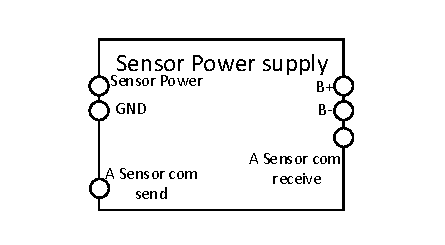
\includegraphics[scale=1]{billeder/CDUSPS}
	\caption{Detailed CDU Sensor Power supply design.}
	\label{fig:CDUSPS}
\end{figure}
Interfaces:
\begin{table}[H]
	\centering
	\begin{tabular}{|p{3cm} |p{3cm} | p{8cm}| }
		\hline
		Interface name: 	&Direction: & Description \\ \hline
		Sensor Power	 &N/A & The Sensor power from the Power supply. \\ \hline
		GND				&N/A & Voltage reference ground. \\\hline 
		A Sensor com send	&Input & Analog sensor communication to bus. \\\hline 
		A Sensor com receive	&Output & Analog sensor communication from bus. \\\hline
		B+ 				&N/A & The B+ input is the positive bus supply connection. \\ \hline
		B- 				&N/A & The B- input is the negative bus supply connection. \\ \hline
	\end{tabular}
\end{table}

\subsubsection{Sensor communication}
The Sensor communication block is responsible for converting digital to analog and analog to digital converting of the signals to and from the sensor nodes. The analog parts are connected to the Sensor Power supply block.
The interfaces to this block can be seen on figure ~\ref{fig:CDUSC}.\\
\begin{figure}[H]
	\centering
	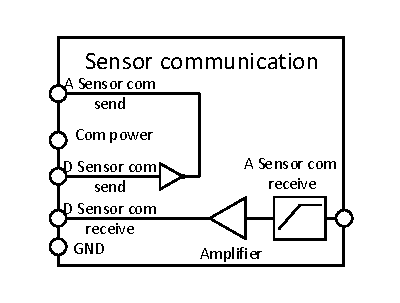
\includegraphics[scale=1]{billeder/CDUSC}
	\caption{Detailed CDU Sensor communication design.}
	\label{fig:CDUSC}
\end{figure}
Interfaces:
\begin{table}[H]
	\centering
	\begin{tabular}{|p{3cm} |p{3cm}| p{8cm}| }
		\hline
		Interface name: & Direction: 	& Description \\ \hline
		Com power	  &N/A & The 3.3V power from the Power supply. \\ \hline
		GND				&N/A & Voltage reference ground. \\\hline 
		A Sensor com send	&Output & Analog sensor communication to bus. \\\hline 
		A Sensor com receive &Input	& Analog sensor communication from bus. \\\hline
		D Sensor com send & Input	& Digital sensor communication from µ-Controller. \\\hline 
		D Sensor com receive &Output	& Digital sensor communication to µ-Controller. \\\hline
	\end{tabular}
\end{table}


\subsubsection{µ-Controller}
The microcontroller block is a hybrid hardware and software block. Software can be found in the software chapter. The hardware part of the µ-Controller block contains the physical pins on the microcontroller.\\
The interfaces to this block can be seen on figure ~\ref{fig:CDUuC}.\\
\begin{figure}[H]
	\centering
	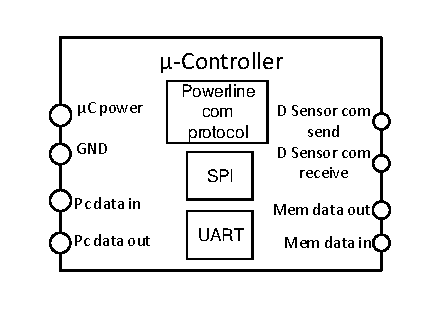
\includegraphics[scale=1]{billeder/CDUuC}
	\caption{Detailed CDU µ-Controller design.}
	\label{fig:CDUuC}
\end{figure}
Interfaces:
\begin{table}[H]
	\centering
	\begin{tabular}{|p{3cm} |p{3cm}| p{8cm}| }
		\hline
		Interface name: & Direction: 	& Description \\ \hline
		µC power	  &N/A & The 3.3V power from the Power supply. \\ \hline
		GND				&N/A & Voltage reference ground. \\\hline 
		D Sensor com send & Output	& Digital sensor communication from µ-Controller. \\\hline 
		D Sensor com receive & Input	& Digital sensor communication to µ-Controller. \\\hline
		Pc data in		&Input & Communication from PC. \\\hline 
		Pc data out		&Output & Communication to PC. \\\hline
		Mem data in		&Output & Data to memory. \\\hline 
		Mem data out	&Input & Data from memory. \\\hline  
	\end{tabular}
\end{table}


\subsubsection{PC communication}
The PC communication block is responsible for converting signals from the levels provided by the microcontroller, from the µ-Controller block, to levels that the PC can understand. The block contains a level converter.\\
The interfaces to this block can be seen on figure ~\ref{fig:CDUPCC}.\\
\begin{figure}[H]
	\centering
	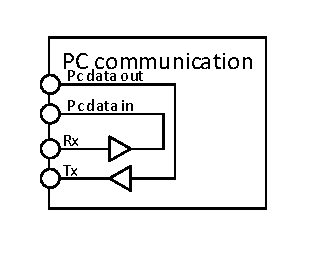
\includegraphics[scale=1]{billeder/CDUPCC}
	\caption{Detailed CDU PC communication design.}
	\label{fig:CDUPCC}
\end{figure}
Interfaces:
\begin{table}[H]
	\centering
	\begin{tabular}{|p{3cm} |p{3cm}| p{8cm}| }
		\hline
		Interface name: & Direction: 	& Description \\ \hline
		Pc data in		&Output & Communication to µ-Controller. \\\hline 
		Pc data out		&Input & Communication from µ-Controller. \\\hline
		Rx		&Input & Communication from PC. \\\hline 
		Tx		&Output & Communication to PC. \\\hline
	\end{tabular}
\end{table}


\subsubsection{Memory}
The Memory block is responsible for storing sensor information and data. The Memory block contains a communication interface and a eeprom or flash memory.\\
The interfaces to this block can be seen on figure ~\ref{fig:CDUM}.\\
\begin{figure}[H]
	\centering
	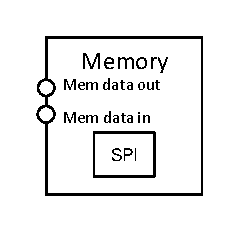
\includegraphics[scale=1]{billeder/CDUM}
	\caption{Detailed CDU Memory design.}
	\label{fig:CDUM}
\end{figure}
Interfaces:
\begin{table}[H]
	\centering
	\begin{tabular}{|p{3cm} |p{3cm}| p{8cm}| }
		\hline
		Interface name: & Direction: 	& Description \\ \hline
		Mem data in		&Output & Data from µ-Controller. \\\hline 
		Mem data out	&Output & Data to µ-Controller. \\\hline  
	\end{tabular}
\end{table}

\subsection{Block construction}
This section describes all detailed calculations done to realize the implementation as well as detailed schematics.\\
\subsubsection{Power Supply}
The Power Supply consist of a voltage regulator block. This block is implemented using a LM317LZ linear voltage regulator. The typical application is found in the data sheet as of figure ~\ref{fig:LM317}. The equation from the datasheet is used to determine the output voltage is given:\\
\begin{equation}
	V_{out}=1.25V\left(1+\frac{R2}{R1}\right)+ I_{ADJ}*R2
\end{equation}
Given is:
\begin{equation}
	R1 = 240\Omega $\\$
	V_{OUT}=3.3V	$\\$
	I_{ADJ}=50 \mu A(typ.)
\end{equation}
Solving for R2 gives us:
\begin{equation}
	R2 \approx 390\Omega
\end{equation}

To determine the input voltage needed on the P+ and P- pins:\\
\begin{equation}
	V_{supply}=5.5V + 5V * n
\end{equation}
Given is n = 2, for 2 sensors used for feasibility testing:
\begin{equation}
	V_{supply}=15.5V
\end{equation}
\begin{figure}[H]
	\centering
	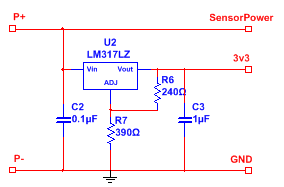
\includegraphics[scale=0.8]{billeder/impps}
	\caption{CDU Power supply implementation}
	\label{fig:CDUimpps}
\end{figure}

\subsubsection{Sensor Power supply}
The Sensor Power supply block consists of constant current generator. The A Sensor com send input allows the constant current generator to assume 2 current values. These are given by the formula extracted from the circuit found in figure ~\ref{fig:ccg}.\\
\begin{figure}[H]
	\centering
	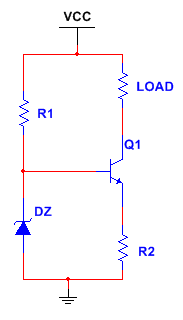
\includegraphics[scale=0.8]{billeder/ccg}
	\caption{Constant current generator}
	\label{fig:ccg}
\end{figure}
The constant current on the bus is found using the following equations:
\begin{equation}
	I_{R2}= \frac{(V_{Zener}-V_{BE})}{R2}
\end{equation}
Given is:
\begin{equation}
	V_{Zener} = 4.8V $\\$
	V_{BE} = 0.65V $\\$
	R2 = 200\Omega
\end{equation}
The current on the bus is:
\begin{equation}
	I_{R2}= 20.75 mA
\end{equation}
In order to open the zener diodes and the transistor we have to dimension the R1. R1 is given by:
\begin{equation}
	R1= \frac{(V_{Supply}-V_{Zener})}{i_{Zener}+K * I_B}
\end{equation}
Given is:
\begin{equation}
	I_{Zener} = 1 mA $\\$
	V_{Supply} = 15.5V $\\$
	V_{Zener} = 4.8V $\\$
	K = 1.2 $\\$
	I_B = 1 mA
\end{equation}
R1 will be:
\begin{equation}
	R1 \approx 5.1k\Omega
\end{equation}
Communication levels are determined by the A Sensor com send input. Toggling a diode nets us a $\Delta$current of:
\begin{equation}
	\Delta I = \frac{0.7V}{200\Omega} = 3.5 mA
\end{equation}
The finished implementation is found in figure ~\ref{fig:CDUimpsps}
\begin{figure}[H]
	\centering
	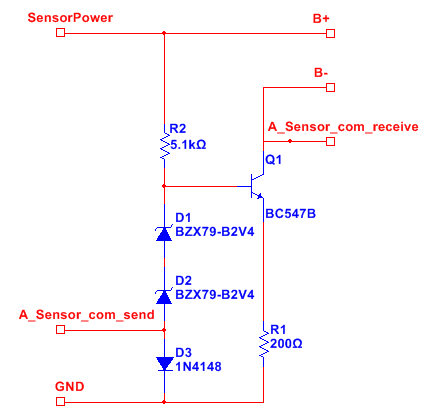
\includegraphics[scale=0.8]{billeder/impsps}
	\caption{CDU Sensor Power supply implementation}
	\label{fig:CDUimpsps}
\end{figure}


\subsubsection{Sensor communication}
The sensor communication block is implemented with 2 functions. The sending part is composed of a digital signal input that opens and closes a transistor. When the digital signal is high, the transistor is open, meaning the bus will have a constant current of 20.75 mA (From Sensor Power supply block). When the digital signal is low, the transistor is closed, meaning the bus will have a constant current of 20.75 mA + 3.5 mA. This in turn means that a high on the input will be low on the bus. Low on the input will be high on the bus. The input is actually inverse.\\
The receiving part is made up of a high pass filter and an amplifier. The levels from the bus will be explained later. For now it will be defined as $\Delta$V = 0.7V. The amplifier is coupled as a comparitor. A voltage reference determines when the output of the amplifier is low and when it is high. The reference is calculted from the following formula:
\begin{equation}
	V_{ref} = 0.430 = \frac{R2}{R1+R2} * V_{in} $\\$
	V_{in} = 3.3V $\\$
	R1 = 100k\Omega $\\$
	R2 = 15k\Omega
\end{equation}
This means when the voltage level on the input of the comparitor is above 0.430, the amplifier output will be high. When below, the amplifier output will be low. The effective gain will be determined by the following formula:
\begin{equation}
	Gain = \frac{V_{out}}{V_{in}} = \frac{3.3V}{0.7V} \approx 5 
\end{equation}
The with a gain of 5, we are well within the Gain Bandwidth Product limit. The Gain Bandwidth Product is defined in the datasheet for the amplifier.\\
The finished implementation is found in figure ~\ref{fig:CDUimpsc}.
\begin{figure}[H]
	\centering
	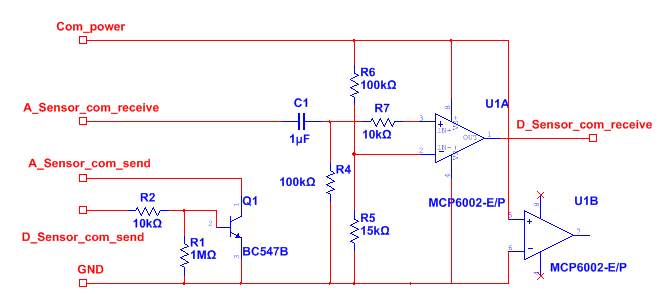
\includegraphics[width=1\textwidth]{billeder/impsc}
	\caption{CDU Sensor communication implementation}
	\label{fig:CDUimpsc}
\end{figure}



\subsubsection{µ-Controller}
The microcontroller block is a hybrid hardware and software block. Software can be found in the software chapter.\\
The PINOUT table for the CDU is found in figure ~\ref{fig:PINOUT}.
\begin{table}[H]
	\centering
    \begin{tabular}{|l|l|l|l|}
    \hline
    Pin name & Pin number & Direction: & Description \\ \hline
    RA4    & 60 & Input          & Send (D Sensor com send)            \\ \hline
    RA5    & 61 & Output          & Receive (D Sensor com receive)    \\ \hline
    RA7	   & 92 & Input			 & UART Test button   \\ \hline
    RF4		& 49 & Input		 & UART Rx \\ \hline
    RF5		& 50 & Output		 & UART Tx \\ \hline
    RD12	& 79 & Output			 & SPI chip select           \\ \hline
    RG6		& 10 & Output			 & SPI clock           \\ \hline
    RG7		& 11 & Input			& SPI MISO		\\ \hline
    RG8		& 12 & Output			& SPI MOSI		\\ \hline
    VSS		& 15 & GND				& Ground for everything \\ \hline
    \end{tabular}
    \caption{PINOUT table for the CDU.}
    \label{fig:PINOUT}
\end{table}


\subsubsection{PC communication}
The PC communication block is a part of the Explorer 16 board. All hardware connections are handled by the board. This means implementation is done solely by software. The hardware connections from the datasheet is found in figure ~\ref{fig:CDUimppcc}.
\begin{figure}[H]
	\centering
	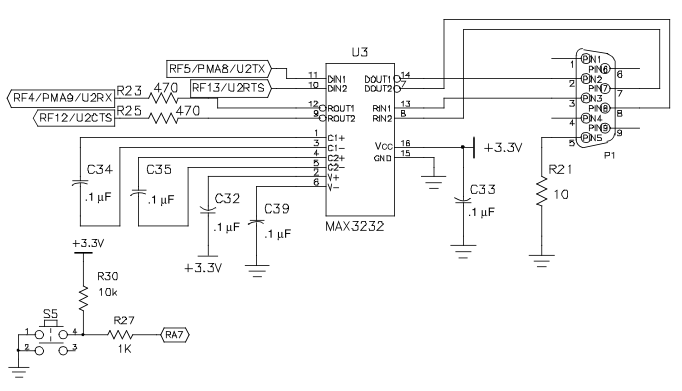
\includegraphics[width=1\textwidth]{billeder/imppcc}
	\caption{CDU PC communication implementation}
	\label{fig:CDUimppcc}
\end{figure}

\subsubsection{Memory}
The Memory block is a part of the Explorer 16 board. All hardware connections are handled by the board. This means implementation is done solely by software. The hardware connections from the datasheet is found in figure ~\ref{fig:CDUimpm}.
\begin{figure}[H]
	\centering
	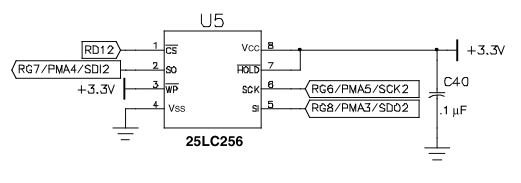
\includegraphics[scale=0.7]{billeder/impm}
	\caption{CDU Memory implementation}
	\label{fig:CDUimpm}
\end{figure}



\section{Sensor Node}
The sensor node responsibility is, as described in the previous documents, to capture a temperature and support the custom powerline communication protocol. Below is described in detail how each block in the sensor node is implemented and designed.

\subsection{Overall design}
Below is shown a figure of the overall sensor node design.
\begin{figure}[H]
\centering
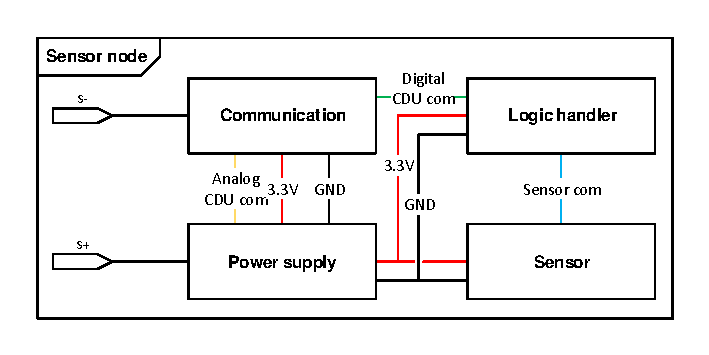
\includegraphics[width=.9\textwidth]{billeder/sn_overall_design}
\caption{Sensor node overall design}
\end{figure}

\subsubsection{Block description}
\textbf{Power supply:}\\
The power supply is creates a steady 3.3V supply to the system from the powerline communication bus.\\

\textbf{Communication:}\\
The communication block convertes the analog communication signal from the CDU to a digital stream of data and clock to the system and the digital communication from the logic handler to an analog signal on the bus to the CDU.\\

\textbf{Logic handler:}\\
The logic handler serves to analyse the incoming data transmission and act accordingly, at the current state this is to either respond with information about the sensor or respond with measured data.\\

\textbf{Sensor:}\\
The sensor part of the sensor node serves as the actual measurement circuit. This has a logical interface to the logic handler.\\

\subsection{Block breakdown}
This section describes the interfaces and the design of each individual block.\\
Below, in figure \ref{fig:SN_detailed}, is shown a detailed overview of the sensor node design. This will be the basis of the block breakdown section.

\begin{figure}[H]
	\centering
	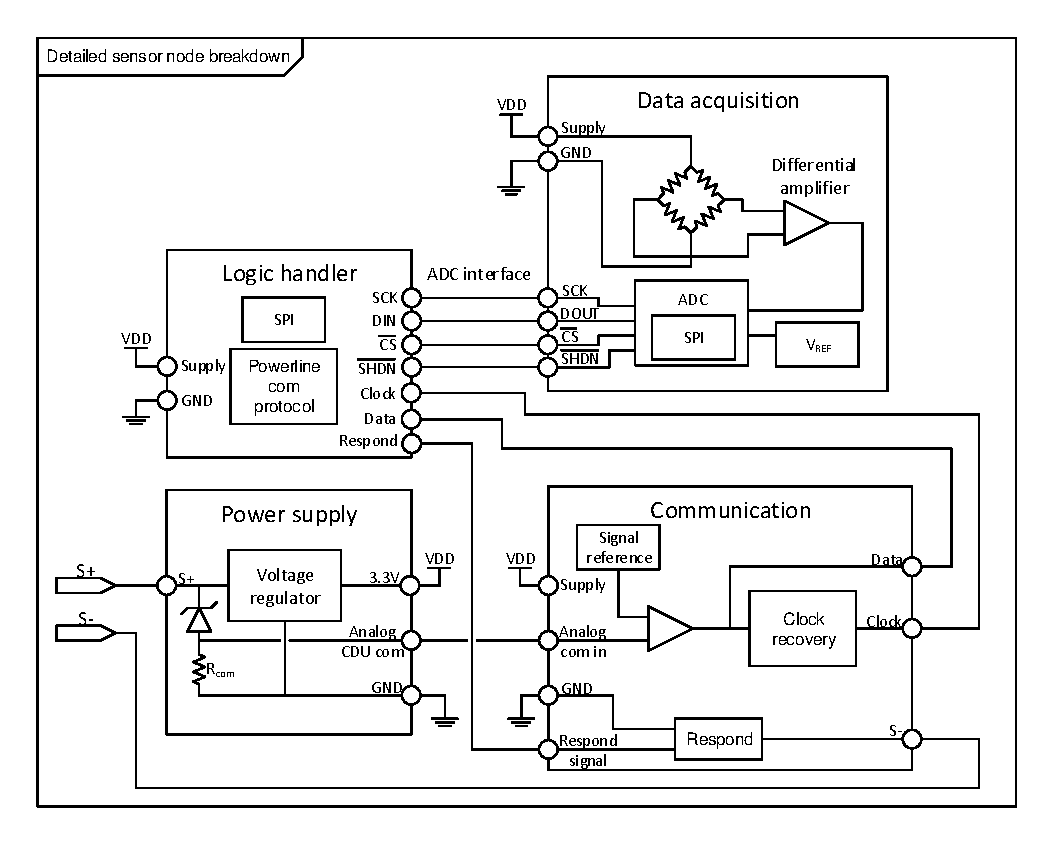
\includegraphics[width=1\textwidth]{billeder/SN_detailed_design}
	\caption{Detailed sensor node breakdown}
	\label{fig:SN_detailed}
\end{figure}

The following subsection will cover all interfaces and design considerations.

\subsubsection{Powersupply}
The power supply block is responsible for power to the entire sensor. This involves making 3.3V to the system in the sensor node and thereby making a reference voltage as ground to the system. Below in figure \ref{fig:SN_PS_FIGURE} is shown the power supply block.

\begin{figure}[H]
	\centering
	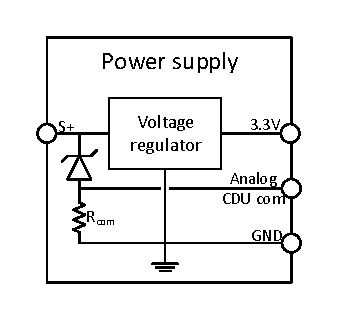
\includegraphics[width=.5\textwidth]{billeder/powersupply_detailed_sn}
	\caption{Sensor node power supply block}
	\label{fig:SN_PS_FIGURE}
\end{figure} 

The goal is to create a steady 3.3V power to the components on the sensor node. The bus is specified as a line where all sensor nodes are placed in series. Therefore each sensor node has an individual reference ground. The line is a constant current modulated with communication.\\
Interfaces:
\begin{table}[H]
	\centering
	\begin{tabular}{|p{3cm} |p{2cm} | p{8cm}| }
		\hline
		Interface name:	& Direction: 		& Description: \\ \hline
		S+ 				& N/A				& The S+ input is the positive connection from the CDU. \\ \hline
		3.3V			& Output			& This is the 3.3V supply voltage to the descrete components on the sensor node. \\ 	\hline
		Analog CDU com  & Output			& The voltage drop caused by the communication current over the communication resistor (R$_{\text{com}}$).\\ \hline
		GND				& N/A				& Voltage reference ground on the individual sensor.\\\hline 
	\end{tabular}
	\caption{Sensor node power supply block interface descriptions}
\end{table}

The S+ and S- signals are from the powerline bus where S+ is connected to the previous sensor or the CDU B+ pin. The S- is connected to the next sensor or the CDU B- pin.\\

The diode and R$_{\text{com}}$ creates a voltage drop from which the voltage regulator creates the steady 3.3V supply. The R$_{\text{com}}$ resistor serves to "convert" the current modulated communication to a voltage to the communication block.

\subsubsection{Communication}

The purpose of the communication block is to synchronize the sensor node clock to the CDU clock to make sure the data is sampled properly.

\begin{figure}[H]
	\centering
	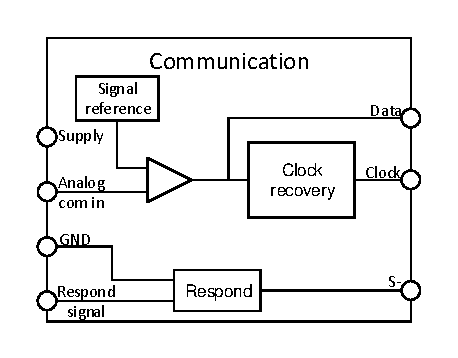
\includegraphics[width=.5\textwidth]{billeder/communication_sn}
	\caption{Sensor node communication block}
	\label{fig:SN_com_fig}
\end{figure}

The communication block generates a steady synchronized clock and converts data to the correct logic levels. It also has a logical interface which enables responds to the CDU by modulating the voltage drop over the entire sensor. In figure \ref{fig:SN_com_fig} the communication block is shown.

\begin{table}[H]
	\centering
	\begin{tabular}{|p{3cm} |p{2cm} | p{8cm}| }
		\hline
		Interface name:	& Direction: 		& Description: \\ \hline
		Supply			& N/A				& 3.3V from the power supply. \\ \hline
		GND				& N/A				& Voltage reference ground on the individual sensor.\\\hline 
		Analog com in	& Input				& The voltage-converted communication signal from the CDU.\\ \hline
		Respond signal  & Input				& Digital input with the respond to the CDU from the logic handler. \\ \hline
		Data			& Output			& Digital output of the incoming data stream from the CDU.\\ \hline
		Clock			& Output			& Clock recovered from the incoming data stream from the CDU. \\ \hline
		S-				& N/A				& The connection out of the sensor node\\ \hline
	\end{tabular}
	\caption{Sensor node communication block interface descriptions}
\end{table}

The Analog CDU com signal received from the powersupply is converted to the correct logic levels on the sensor node. This is done with an amplifier and a signal reference. The converted signal is now a direct image of the data transmitted from the CDU. The clock recovery circuit is responsible for creating a synchronized clock from this data signal. The respond circuit receives logic levels from the logic handler and generate an analog signal which is received at the CDU.

\subsubsection{Logic handler}
The logic handler is the central computational unit and is a programmable logic chip. It serves to interpret incoming messages and act accordingly whilst also interfacing with the ADC to acquire new data to be sent to the CDU. In figure \ref{fig:sn_logic_handler} the logic handler block is shown.

\begin{figure}[H]
	\centering
	\includegraphics[width=.5\textwidth]{billeder/logic_handler_sn}
	\caption{Sensor node logic handler block}
	\label{fig:sn_logic_handler}
\end{figure}

\begin{table}[H]
	\centering
	\begin{tabular}{|p{3cm} |p{2cm} | p{8cm}| }
		\hline
		Interface name: 			& Direction: 	& Description: \\ \hline
		Supply						& NA			& 3.3V from the power supply. \\ \hline
		GND							& NA			& The voltage-converted communication signal from the CDU.\\ \hline
		Respond		  				& Output		& Digital respond signal to the respond circuit in the communication block. \\ \hline
		Clock						& Input			& 20kHz synchronized clock from the communication block.\\\hline 
		Data						& Input			& Digital data from the communication block.\\\hline
		SCK							& Output		& Serial clock to the SPI interface to the Data acquisition block.\\\hline
		DIN							& Input			& Data received from the Data acquisition block.\\\hline
		$\overline{\text{CS}}$		& Output		& Active low chip select to the Data acquisition block.\\\hline
		$\overline{\text{SHDN}}$	& Output		& Active low shutdown input on the Data acquisition block.\\\hline
	\end{tabular}
	\caption{Sensor node logic handler block interface descriptions}
\end{table}

The incoming message is received by the scheme described in the architecture section regarding the protocol. The logic handler shift between several states to accommodate the functionality described in the architecture. These states makes sure the sensor are able to decode the incoming messages correct and the respond with the right message corresponding to the function code. 

\begin{figure}[H]
	\centering
	\includegraphics[width=1\textwidth]{billeder/logic_handler_stm}
	\caption{Sensor node logic handler state machine}
\end{figure}

The state machine controller state machine checks incoming data for the right pattern. When the start sequence is received it changes the state to "check address" in the state machine controller state machine and "Manchester converting" in the Line coding state machine. If the correct address is received the state machine controller state machine then changes its state to "Check function code", lastly, depending on the function code, the state machine controller state machine prepares the data to be sent in the response. The state machine controller state machine then changes the state of the Line coding state machine to the "Respond" state and goes into the "Idle" state.\\
The Line coding state machine samples all data in an 8 bit buffer in the idle state. This buffer is used in the idle state of the state machine controller. If this matches the start sequence the state is changed to "Manchester converting". This state handles the manchester decoding of the incoming stream of data. The first four manchester bits is then stored in an address buffer. If this address corresponds to the sensor nodes address then next four manchester bits are stored in a function code buffer. If this fits within the known function code the respond data buffer is filled with the corresponding data and the line coding state machine state is changed to the Respond state. The respond state serially runs through the respond data buffer as the clocks ticks in.\\

The physical structure of the logic handler is divided into two parts. One which handles the power line communication bus and one the handles the interface with the data acquisition block. These two parts are then interconnected and the power line communication bus flops the data from the data acquisition interface block when it is not sampling new data. The conversion from ADC steps to actual temperature is handled in the data acquisition interface block.

\subsubsection{Data acquisition}

The data acquisition block handles physical measurements of temperature and has a digital interface to the logic handler. It's comprised of a measurement bridge, a differential amplifier and an ADC.

\begin{figure}[H]
	\centering
	\includegraphics[width=.5\textwidth]{billeder/data_aqcuisition_sn}
	\caption{Sensor node data acquisition block}
	\label{fig:sn_data_acquisition}
\end{figure}

\begin{table}[H]
	\centering
	\begin{tabular}{|p{3cm} |p{2cm} | p{8cm}| }
		\hline
		Interface name: 			& Direction: 	& Description: \\ \hline
		Supply						& NA			& 3.3V from the power supply. \\ \hline
		GND							& NA			& The voltage-converted communication signal from the CDU.\\ \hline
		Respond		  				& Output		& Digital respond signal to the respond circuit in the communication block. \\ \hline
		SCK							& Input			& Serial clock from the logic handler block.\\\hline
		DOUT						& Output		& Data from the ADC to the logic handler block.\\\hline
		$\overline{\text{CS}}$		& Input			& Active low chip select.\\\hline
		$\overline{\text{SHDN}}$	& Input			& Active low shutdown input from the logic handler block.\\\hline
	\end{tabular}
	\caption{Sensor node data acquisition block interface descriptions}
\end{table}

The measurement bridge is powered by the 3.3V supply. The bridge should be balanced at a low enough temperature so data isn't lost if the actual temperature is lower than this, the gain in the differential amplifier must not exceed so the maximum temperature measurement is too low of what would be expected. Due to low power at our disposal the bridge must not draw too much current.\\
The voltage measurement is performed by an ADC with an external voltage reference and a SPI [1] like interface.

\subsection{Block construction}
This section describes all detailed calculations done to realize the implementation aswell as detailed schematics.\\

\subsubsection{Power supply}
As seen on figure \ref{fig:SN_PS_FIGURE} the power supply consists of a zener diode, a sense resistor and a voltage regulator.\\
The voltage regulator should output a 3.3V to supply the sensor. Below on figure \ref{fig:LM317} is shown a typical application from the datasheet. The to this application the following formula for output voltage is given:\\
\begin{equation}
	V_{out}=1.25V\left(1+\frac{R2}{R1}\right)+ I_{ADJ}*R2
\end{equation}

With R1 given as 240$\Omega$, V$_{OUT}$=3.3V and I$_{ADJ}$=50$\mu$A(typ.) R2 will be $\approx$ 390$\Omega$.


\begin{figure}[H]
	\centering
	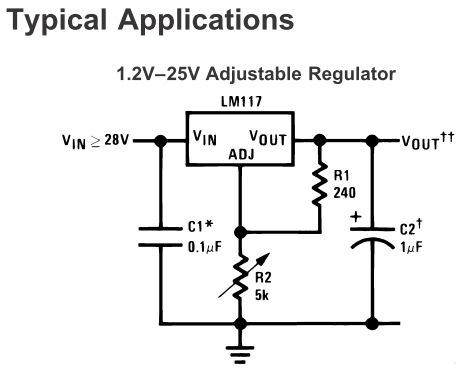
\includegraphics[width=.5\textwidth]{billeder/LM317}
	\caption{LM117 voltage regulator series typical application}
	\label{fig:LM317}
\end{figure}

In the datasheet the input voltage versus output voltage is specified to a minimum of 3V to ensure the specified output current of 100mA. But since we doesn't need more then 20mA at max we tested the regulator with $V_{IN}-V_{OUT}=1.3V$ and the output voltage is well within acceptable levels.\\
The sense resistor is placed in series with the diode. The resistor serves to "convert" the current modulated communication to a voltage signal. The current level change for a 0 and a 1 the CDU is specified to 3.5mA. A communication resistor of $\sim$ 5$\Omega$ is chosen. Therefore a logical 0 will be a voltage drop $5\Omega * 20.5mA = 103mV$ and a logical 1 will be have a drop of $5\Omega * 24mA = 120mV$. The communication will therefore have $\Delta V=17mV$. This analog signal is connected to the input of the communication block for further conversion.\\
\textbf{Simulation result:}

\begin{figure}[H]
	\centering
	\includegraphics[width=.5\textwidth]{billeder/PS_lm317_sim}
	\caption{Powersupply simulation}
	\label{fig:ps_sim}
\end{figure}

\subsubsection{Communication}
As seen on figure \ref{fig:SN_com_fig}, the communication block comprises of an amplifier, a signal reference, a clock recovery circuit and a respond circuit. Each block will be described here.\\
\textbf{Amplifier and signal reference:}\\
The amplifier serves to amplify the received signal to logic levels. On the sensor node logic levels are 0 ($\sim$ 0V) and 1 ($\sim$ 3.3V). Therefore a rail-to-rail amplifier is chosen. The amplifier comprises of a two step amplification, the first one amplifies the raw signal and the second amplifies the signal with reference to the filtered signal (averaged signal). Below on figure \ref{fig:communication_amplifier_circuit} is shown the implementation:

\begin{figure}[H]
	\centering
	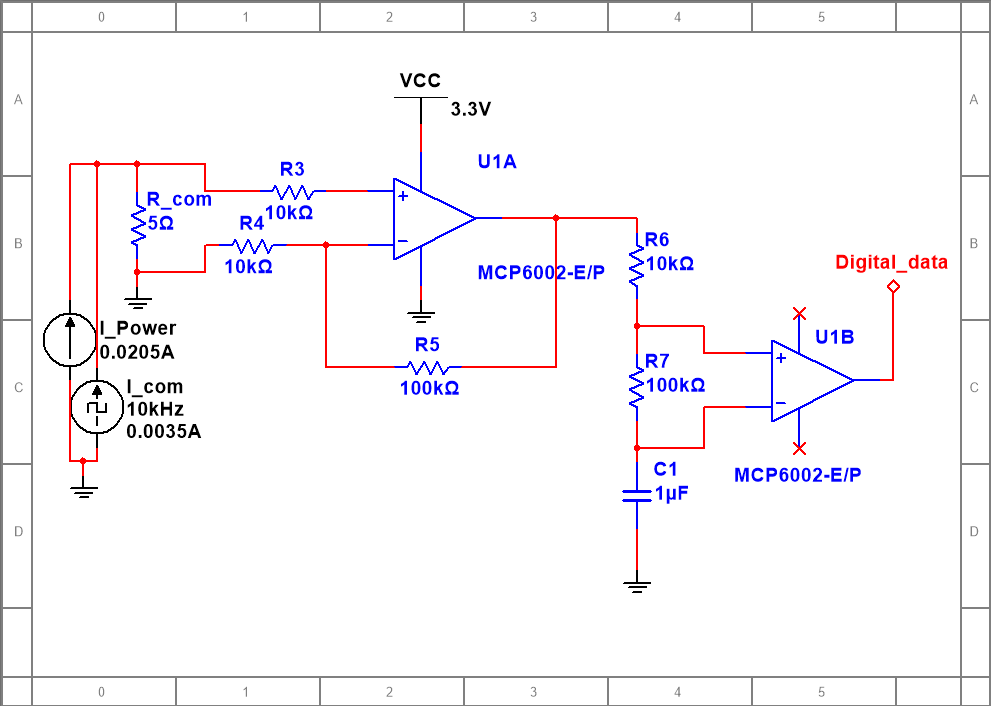
\includegraphics[width=.6\textwidth]{billeder/communication_amplifier_sn}
	\caption{Communication amplifier circuit}
	\label{fig:communication_amplifier_circuit}
\end{figure}

After the first amplifier $\Delta V$ is amplified by the gain factor(k):
\begin{equation}
	k=\frac{100k\Omega+10k\Omega}{10k\Omega}=11
\end{equation}
Therefore $\Delta V=k*17mV=187mV$. The signal is then averaged by the filter comprised of R7 and C1 (see figure \ref{fig:communication_amplifier_circuit}) and the operation amplifier works as a comparator. The comparator amplifies the signal from 187mV to rail ($\sim$3.3V) when the signal is high and to ground ($\sim$0V) when the signal is low. The comparator gains the signal $\frac{3.3V}{120mV*k}\approx 2.5$ when it is high.\\
This is done because of the slew rate of the operation amplifier MCP6002 wasn't sufficient. The MCP6002 series was the available rail-to-rail operation amplifier.\\
According to the calculations the slew rate should be sufficient but after testing the design the decision was made to make it a two stage amplifier.
Slew rate calculation:
\begin{equation}
	F_{MAX}=\frac{0.6\frac{V}{\mu s}}{2*\pi*3.3V}\approx29kHz
\end{equation}

\textbf{Clock recovery:}\\
The clock recovery circuit comprises of a Phased lock loop (PLL) and a clock divider (JK flip flop). The PLL consists of a phase detector (PD), a voltage controlled oscillator (VCO) and a loop filter. The PLL's purpose is to lock on the frequency of the incomming data, and then providing a steady clock to sample the received data. The PLL is a CD4046BE from texas instruments. Below, in figure \ref{fig:cd4046} is shown the block diagram for the CD4046.

\begin{figure}[H]
	\centering
	\includegraphics[width=.6\textwidth]{billeder/CD4046}
	\caption{CD4046 block diagram}
	\label{fig:cd4046}
\end{figure}

In this design the phase comparator (PD) type 1 is used. It is basically an x-or gate comparing the two input clock. If the two clock are logically different the PD sends a high output and if the two input clocks are logically equal it sends a low output. The output of the PD is then filtered with a low pass filter and fed to the input of the VCO. If the CD4046 is in lock the input to the VCO should be V$_{\text{DD}}$/2. This means when the PLL is locked with PD type 1 it will be in exactly 90$^{\circ}$deg phase. By using a clock divider the logic handler can sample the incoming data
on each rising edge following the waveforms shown in figure \ref{fig:cd4046waveforms} below.

\begin{figure}[H]
	\centering
	\includegraphics[width=.7\textwidth]{billeder/cd4046waveforms}
	\caption{clock and data waveform scheme}
	\label{fig:cd4046waveforms}
\end{figure}

The PLLs VCO is configured by the values of C1, R1 and R2 but also the filter comprised of C2 and R3 impacts the loop.\\
The C1, R1 and R2 component define the frequency lock range. This range is the total range of the VCO meaning it can lock from f$_{\text{max}}$-f$_{\text{min}}$=2f$_{\text{l}}$, the VCO outputs f$_{\text{min}}$ when VCO in = V$_{\text{SS}}$ and f$_{\text{max}}$ when VCO in = V$_{\text{DD}}$. The filter then defines the frequency capture range. This is the range where the PLL will automatically lock if the input frequency is within this span. On figure ... the relation between VCO in and VCO out is illustrated.

\begin{figure}[H]
	\centering
	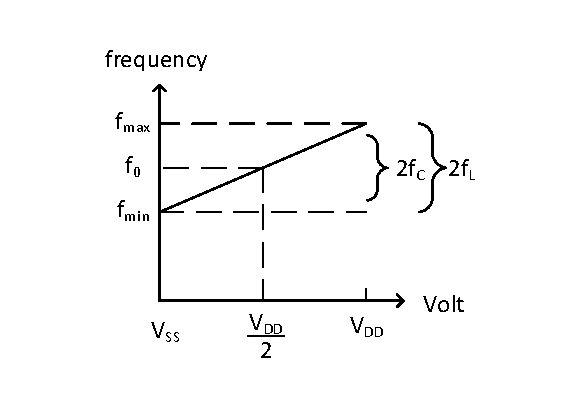
\includegraphics[width=.7\textwidth]{billeder/VCO_graph}
	\caption{VCO voltage in vs. VCO frequency out}
\end{figure}

The first step when dimensioning the VCO is to determine f$_{\text{min}}$. Here we know f$_{\text{min}}$=f$_{\text{0}}$-f$_{\text{l}}$. I this case f$_{\text{0}}$=20kHz since we have a clock divider and f$_{\text{l}}$ is chosen to 4kHz. Therefore f$_{\text{min}}$=16kHz. In the datasheet the a graph is provided, see figure \ref{graph:C1}, to dimension the capacitor with regards to R2 and f$_{\text{l}}$, R2=100k$\Omega$.

\begin{figure}[H]
	\centering
	\includegraphics[width=.7\textwidth]{billeder/c1_graph_cd4046}
	\caption{C1 dimension graph CD4046}
	\label{graph:C1}
\end{figure}

The capacitor should be in the 1nF area but as seen on the graph the variation in components can vary as much as 15\% operating at 5V, and since the sensor node is running at 3.3V a large variation is expected. When the capacitor is determined R1 is the last component. R1 is determined with the relation f$_{\text{max}}$/f$_{\text{min}}$ versus R2/R1 as seen on figure \ref

\begin{figure}[H]
	\centering
	\includegraphics[width=.7\textwidth]{billeder/}
\end{figure}




So to determine the correct capacitor a "trial and error" method is used. When there are no frequency on the input signal (of the PD) the VCO will output f$_{\text{0}}$.

\subsubsection{Logic handler}

\subsubsection{Sensor}



\subsection{Power consumption}


\subsection{Print layout}






